\section{Ver le NewSQL la base de données moderne}
NewSQL est un stockage distribué et potentiellement entièrement en mémoire et pouvant être requêté classiquement par une interface SQL. NewSQL est tiré du monde NoSQL mais reste différent. Comme NoSQL il s’agit d’une nouvelle architecture logicielle qui propose de repenser le stockage des données. Elle profite des architectures distribuées, des progrès du matériel et des connaissances théoriques depuis 35 ans. Mais contrairement à NoSQL elle permet de conserver le modèle relationnel au coeur du système.

NewSQL est né de la rencontre de 3 types d’architecture, relationnelle, non-relationnelle et grille de données appelée également cache distribué, comme indiqué dans la Figure ci-dessous. En effet il se positionne comme un stockage distribué conçu dans le prolongement des architectures NoSQL, pour des accès transactionnels à fort débit, au moyen d’une interface SQL. D’un point de vue évolutivité, il se situe en tant que concurrent direct des solutions NoSQL. Mais contrairement à ces solutions il conserve une interface relationnelle via le SQL, ce qui est l’une de ses forces. Enfin la plupart des solutions NewSQL proposent un stockage en mémoire. Ce stockage en mémoire distribué sur plusieurs machines sous forme de grille de données est largement utilisé depuis une dizaine d’années dans les environnements où une faible latence est critique, notamment dans certaines applications des banques d’investissement. Les solutions NewSQL partagent ainsi un positionnement intermédiaire entre les solutions NoSQL et les grilles de données.

\begin{figure}[h]
	\centering
    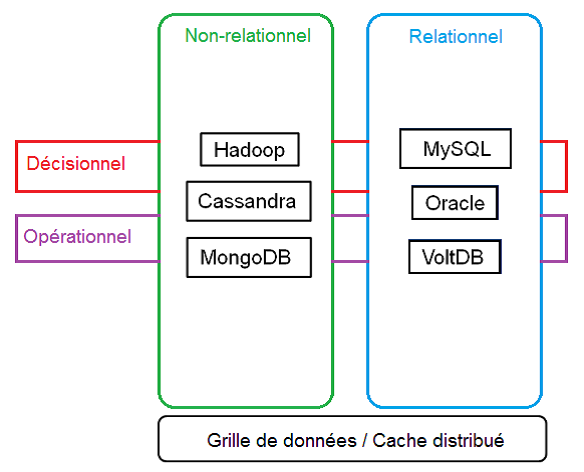
\includegraphics[scale=0.5]{img/part1/4.13}
    \caption{Naissance du NewSQL à partir de 3 architectures}
\end{figure}
\newpage
\subsection{L’architecture NewSQL :}
L’architecture NewSQL reprend des expériences antérieures du SQL relationnel et du NoSQL plusieurs caractéristiques, tout en ayant certaines particularités en termes de choix et d’avantages : 
\begin{enumerate}
\item Le choix d’une interface SQL et d’un schéma relationnel. 
\item Le schéma relationnel avec des limitations pour faciliter la distribution des données et des traitements. 
\item La distribution et la réplication des données pour assurer l’évolutivité et la résilience. 
\end{enumerate}

\begin{figure}[h]
	\centering
    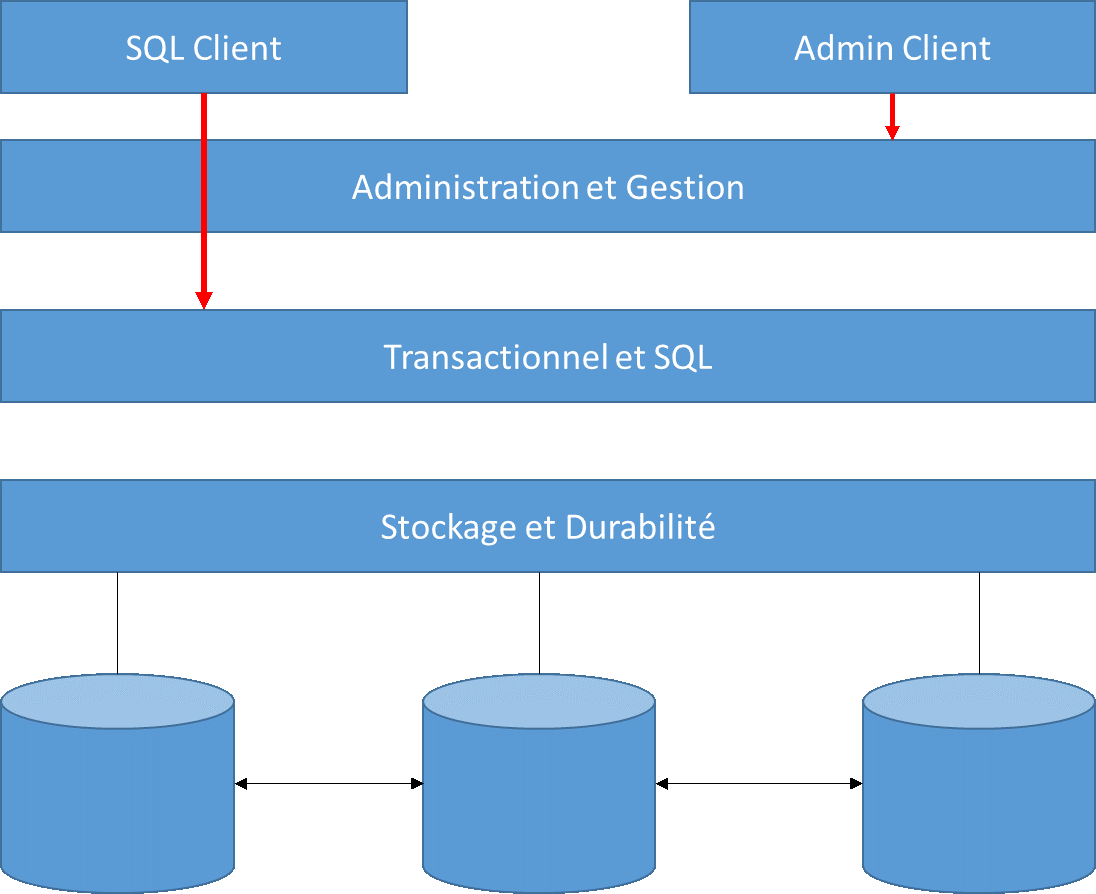
\includegraphics[scale=0.5]{img/part1/4.14}
    \caption{L'architecture d'une base de données NewSQL populaire NueDB.}
\end{figure}

\subsection{Les avantages de la solution NewSQL :}
La solution NewSQL présente des avantages intéressants en termes de performances par rapport à ses prédécesseurs : 
\begin{enumerate}
\item Elle utilise le SQL comme langage commun de requêtes. 
\item Elle présente une architecture qui a de meilleures performances par noeud que les solutions classiques \item type SGBD relationnel. 
\item Elle minimise la complexité des applications tout en améliorant la consistance des données et en fournissant un support transactionnel complet. 
\item Elle est compatible avec les outils de travail du standard SQL. 
\item Elle fournit des analyses plus riches des traitements. 
\item Elle est compatible avec l’architecture distribuée des Clusters. 
\item Elle fournit un traitement plus performant des données en mémoire. 
\end{enumerate}

\newpage
\subsection{Les limites de la solution NewSQL :}
La solution NewSQL est confrontée à quelques limitations l’empêchant d’atteindre un niveau de maturité suffisant :
\begin{enumerate}
\item Son architecture de calcul en mémoire, dit In-Memory, ne fonctionne pas au-delà de quelques TO de données.
\item Cette architecture nécessite un matériel spécifique avec des capacités importantes de stockage en mémoire, ce qui revient très onéreux.
\item Malgré son attitude à vouloir intégrer le modèle relationnel, le NewSQL fournit un accès limité aux outils de travail du standard SQL.
\end{enumerate}

\subsection{Résumé :}
Une base de données NewSQL conserve la structure classique en colonnes mais fait appel à différents procédés pour conserver la rapidité même sur de larges volumes. En revanche, cette technologie n’a pas le recul suffisant pour aller plus loin et n'a pas encore pu suffisamment faire ses preuves. Par conséquent les entreprises sont encore réticentes à l'adoption de cette toute nouvelle architecture.

\subsection{Exemples des bases de données NewSQL:}
\textbf{NuoDB :} C'est un SGBD distribué qui pourrait être décrit comme une base de données à faible latence. Il permet à l'utilisateur d'interagir avec lui de manière transactionnelle en prenant en charge les opérations ACID et la réplication des données. 

\begin{figure}[h]
	\centering
    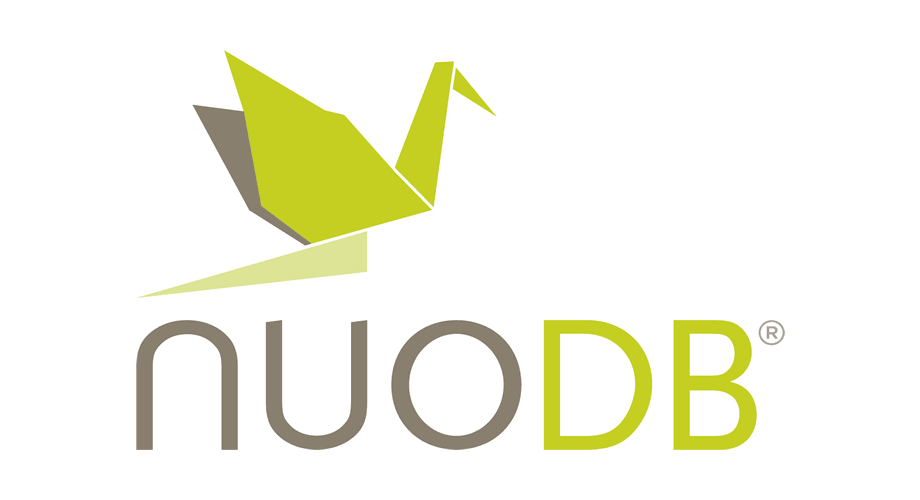
\includegraphics[scale=0.2]{img/part1/4.15}
    \caption{Logo NuoDB.}
\end{figure}


\textbf{VoltDB :} Il s'agit d'une base de données distribuée en mémoire qui est considérablement plus rapide que les bases de données SQL. C’est une base de données flexible qui prend en charge le stockage JSON. Il est le mieux adapté aux applications à lecture fréquente et à faible fréquence d'écriture.

\begin{figure}[h]
	\centering
    
\includegraphics[scale=0.2]{img/part1/4.16}
    \caption{Logo VoltDB.}
\end{figure}

\textbf{Clustrix :} c'est une base de données distribuée qui prend en charge l'analyse en temps réel, elle est optimisée pour les transactions massives. Il prend en charge certains outils de BI 23 et une récupération rapide des données.

\begin{figure}[h]
	\centering
    
\includegraphics[scale=0.1]{img/part1/4.17}
    \caption{Logo Clustrix.}
\end{figure}





